% Chapter Template

\chapter{Bidirectional Grounding of Real Data} % Main chapter title

\label{Chapter6} % Change X to a consecutive number; for referencing this chapter elsewhere, use \ref{ChapterX}

\lhead{Chapter 6. \emph{Bidirectional Grounding of Real Data}} % Change X to a consecutive number; this is for the header on each page - perhaps a shortened title

%----------------------------------------------------------------------------------------
%	SECTION 1
%----------------------------------------------------------------------------------------
\section{The Difficulties of Real Data}
In the previous chapter I showed that it is possible to use a MAE to bidirectionally ground natural language (words) and the visual attributes of images of different objects through MRL. However, the data used in the previous chapter is artificial and therefore many of the challenges which real data presents are not present in it. 

When working with real images, there are many factors to consider such as lighting changes, perspective changes and camera noise \ref{keller2016analysis}. These factors were not present in the ArtS dataset, so in this chapter I will show how these impact MRL for bidirectional grounding.

\section{Acoustic Packaging}
In order to make use of MRL on a robot, it is necessary to have a method to gather and group data from multiple sensory modalities. To do this, I make use of Acoustic Packaging (AP) \cite{schillingmann2009towards, schillingmann2009computational}.

The acoustic packager I implemented for this, is triggered to capture data when sound above a certain threshold is heard by a microphone. Images and audio are recorded with the audio being passed to an Automatic Speech Recogniser (ASR) to transcribe any speech. The audio, transcription and image together are refered to as an acoustic-package.


\begin{figure}[h]
    \centering
    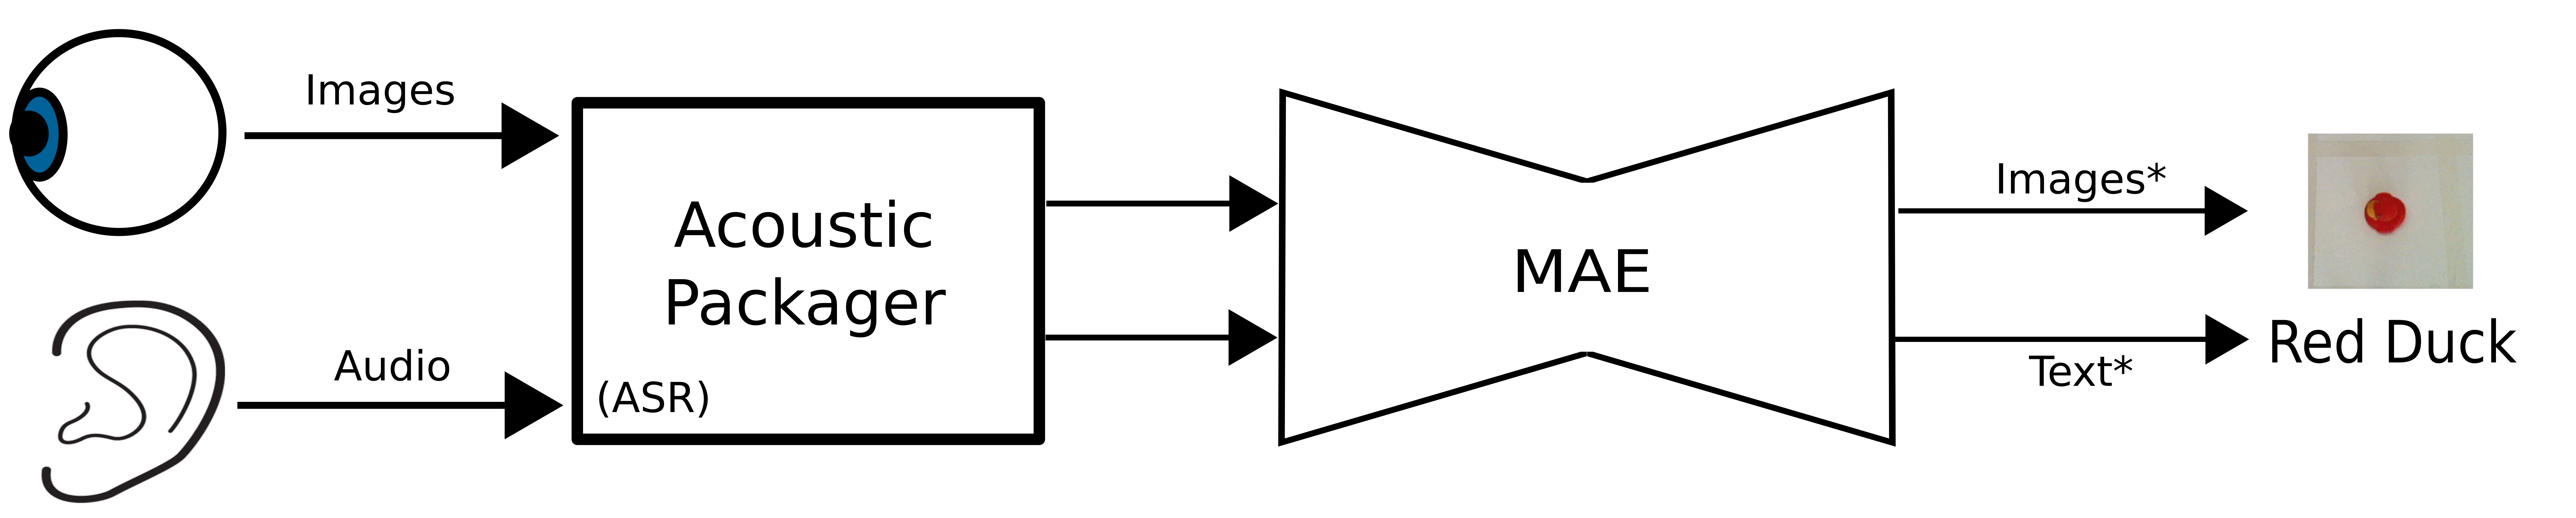
\includegraphics[width=0.7\textwidth]{Figs/chapter6/bimodal_system_schematic.png}
    \caption{System schematic. Data is captured from sensors by an acoustic packager and fed to the multimodal autoencoder (MAE).}
    \label{fig:schematic}
\end{figure}

I do not make use of the audio, I use only the transcribed text and images such that the data used in this chapter is analigous to the data used in the previous chapter.

\section{Real Shapes Dataset}
The Real Shapes dataset (ReShape) was created by presenting various objects to a webcam in 9 different positions and giving a short description of the object. \autoref{fig:Reshape} shows example images from ReShape.

\begin{figure}[h]
    \centering
    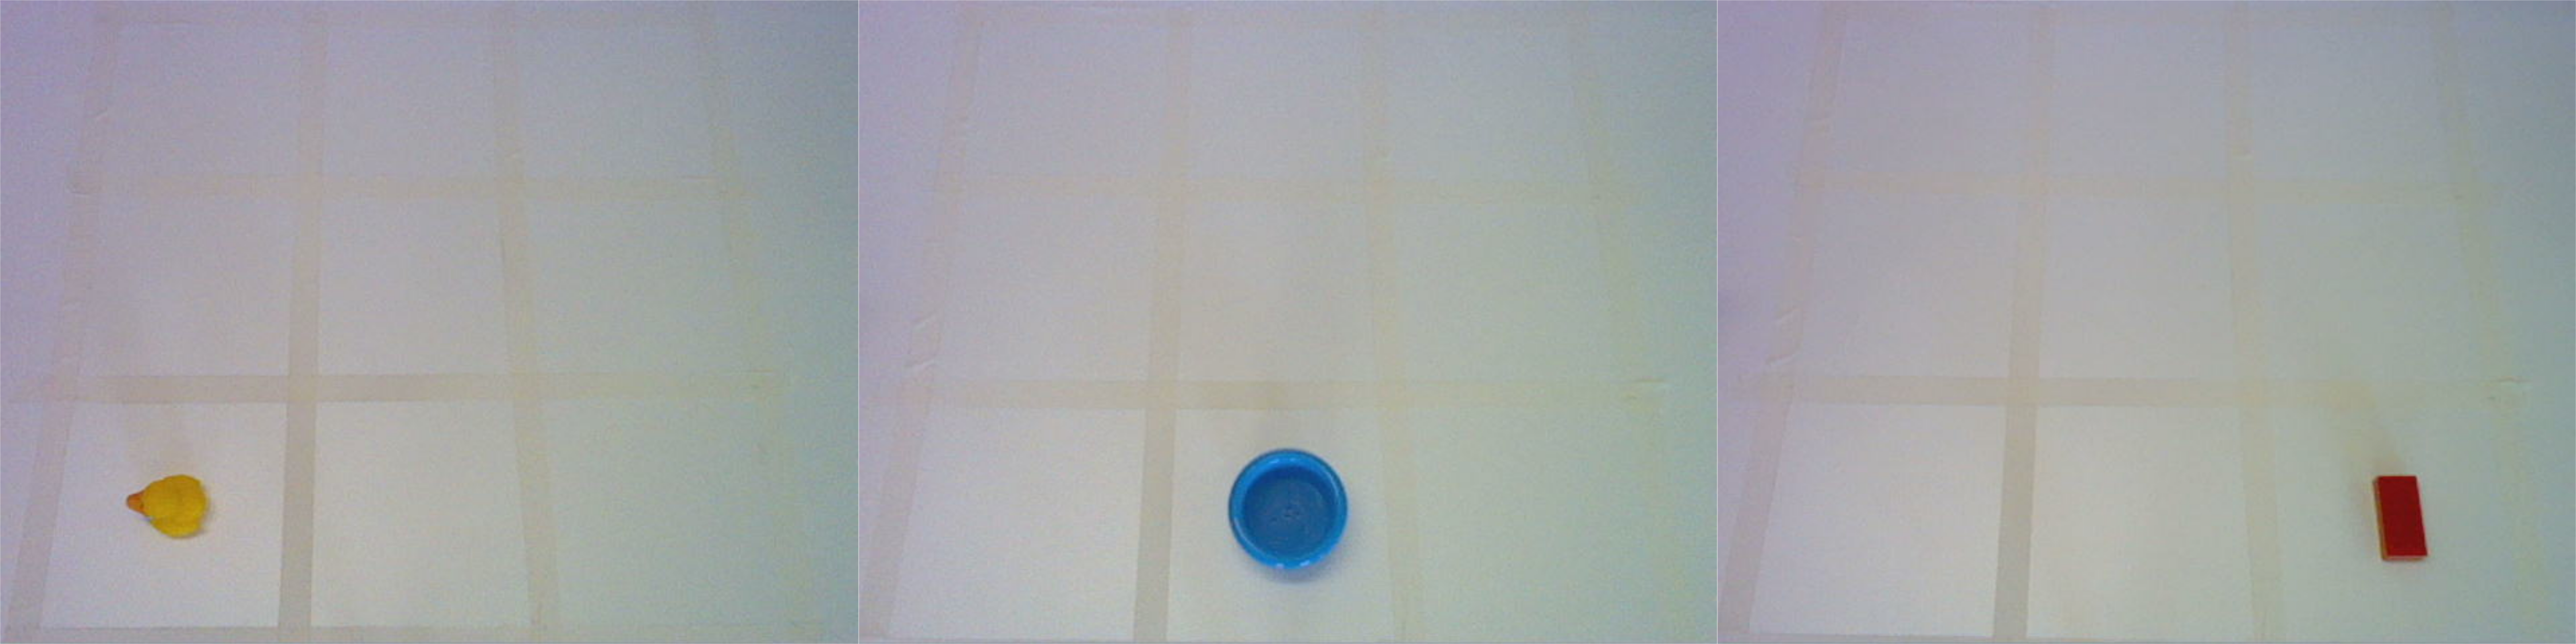
\includegraphics[width=\textwidth]{Figs/chapter6/ReShapeExs.png}
    \caption{Example images from ReShape.}
    \label{fig:ReShape}
\end{figure}


\subsection{Dataset Description}
The ReShape dataset contains images and short descriptions of the images.

There are 7 objects, in 10 colours and 3 sizes. Not all objects have appear in all 10 colours or all 3 sizes.


\subsection{Problem Description}
As in the previsous chapter I will be training the MAE to learn a joint embedding of images and their descriptions. The descriptions only contain a size, shape and colour and not a position as the images are cropped, centring the object in the image, the notion of position is removed from both modalities.

\subsection{Network Description}
I make use of the same network as used in chapter 4 with an embedding size of 296 neurons. 

\section{Experiments with the Reshape dataset}
In the following experiments I do not consider the notion of position and instead crop each image so that the object is roughly centred and consider all objects of the same type to be the equivalent regardless of position (e.g. a ``big blue duck top left'' is considered the same as a ``big blue duck center''). As such, the position word is removed from the description of the image and the MAE does not contain the position words in its "vocabulary".

\begin{figure}[h]
    \centering
    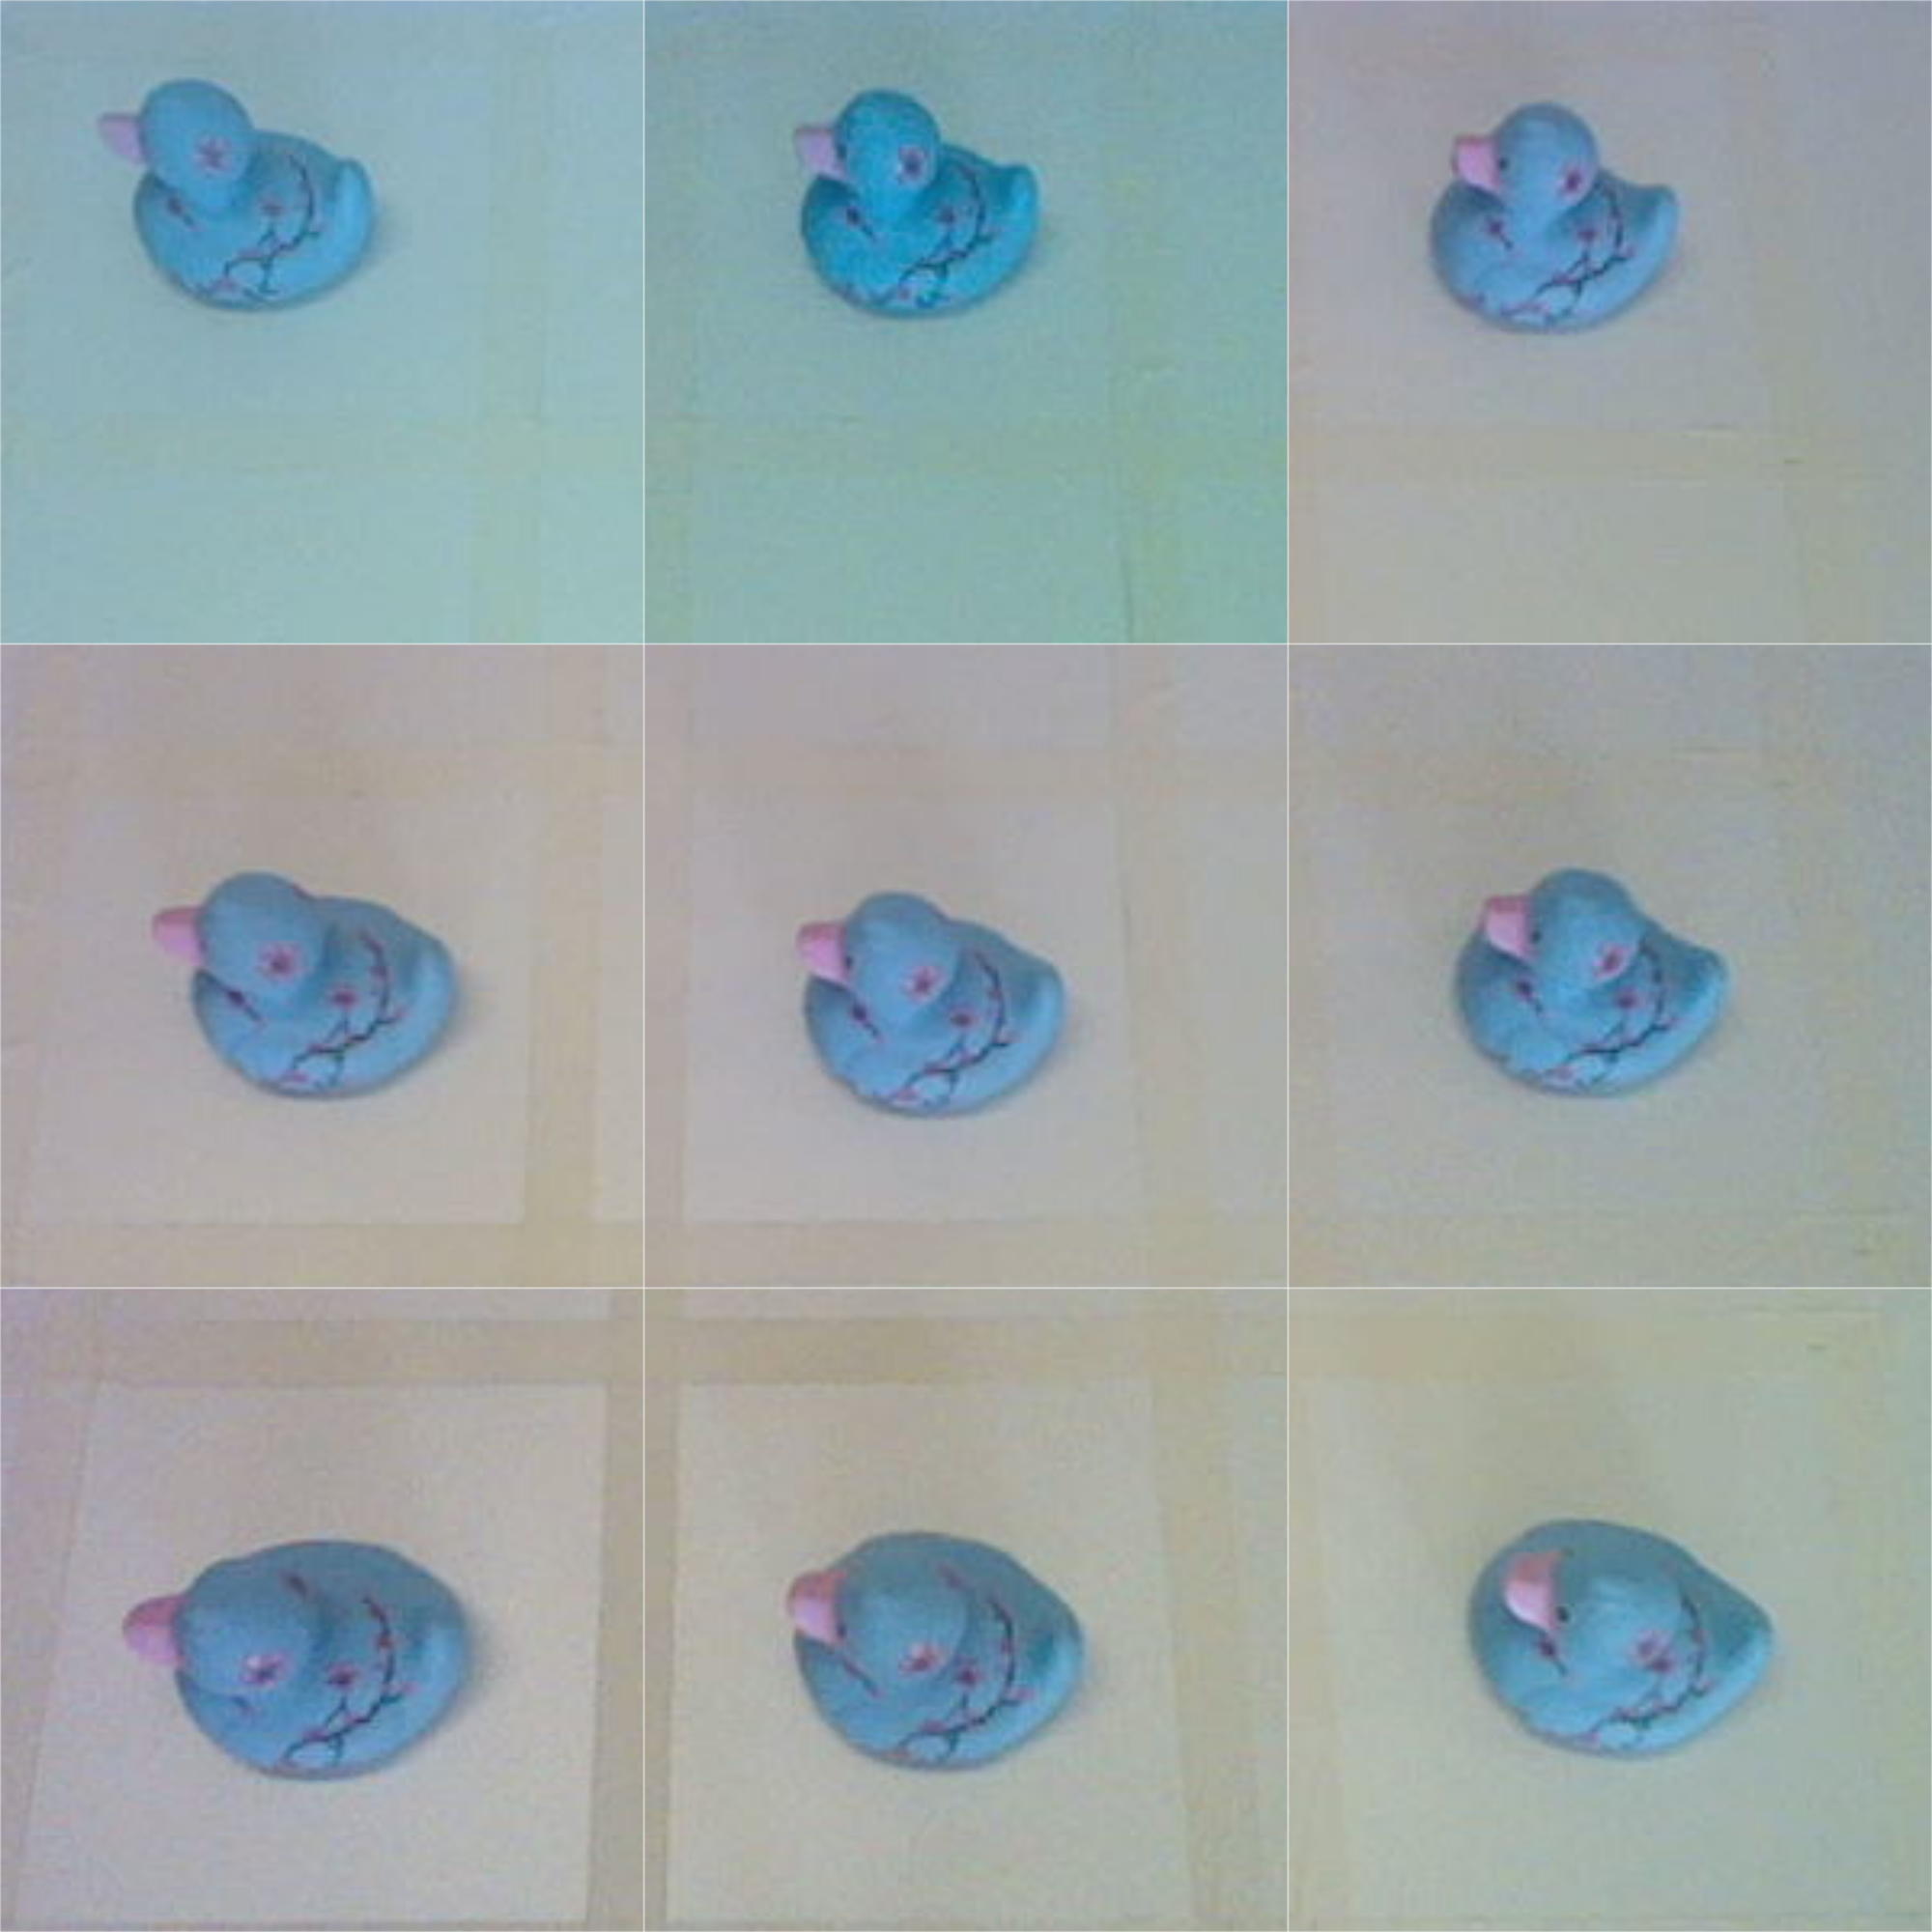
\includegraphics[width=0.7\textwidth]{Figs/chapter6/ReShapeCrop.png}
    \caption{Example cropped images from ReShape.}
    \label{fig:ReShapeCrop}
\end{figure}

Cropping the images is done for three main reasons. 1) this increases the amount of training data for each object by a factor of nine. As the notion of position is removed, the same object in a different position is no longer considered a separate object (unlike in the previous chapter). 2) Cropping reduces the amount of the MAEs field of view which contains the background. This should make it easier for the MAE to learn the visual attributes of the objects as less computation is wasted processing the background. 3) Cropping greatly reduces the necessary computation to process a single image as the images are much smaller. Cropping does this without reducing the size of the object in the image unlike resizing the raw image.

Cropping is performed heuristicly, using the position word from the image description to crop out a predefined region. \autoref{fig:CropHeur} shows the regions that each position word relates for the purposes of cropping.

\begin{figure*}[ht]
    \centering
    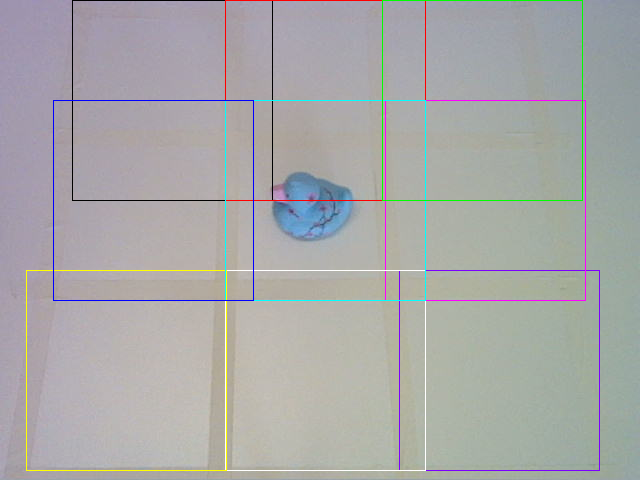
\includegraphics[width=0.7\textwidth]{Figs/chapter6/cropHeuristics.png}
    \caption{Regions to crop to given different postion words.}
    \label{fig:CropHeur}
\end{figure*}


%After cropping, their are changes in the visual attributes of the images which are not accounted for in their descriptions. For example, images in top positions, were further from the camera so they appear slightly smaller than those in bottom positions.

Calculating the average image for each objectprovides insight into what to expect when generating images in the Words Only condition. As the MAE is trained to optimise the MSE of its output with respect to the training data, in the Words Only condition, the best images for it to generate are the average images for each object.


\begin{figure*}[ht]
    \centering
    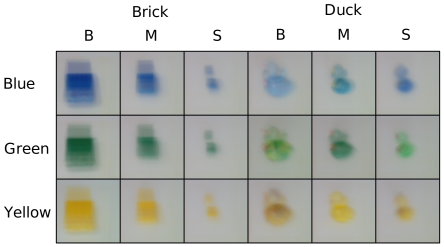
\includegraphics[width=0.7\textwidth]{Figs/chapter6/avgBrickDuckBGY.png}
    \caption{Average images of bricks and ducks in different sizes and colours.}
    \label{fig:AvgBrickDuck}
\end{figure*}

\begin{figure*}[ht]
    \centering
    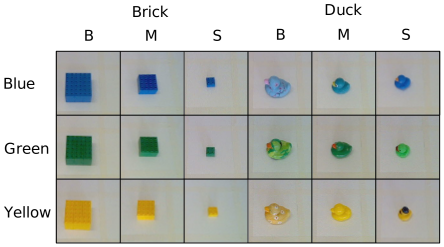
\includegraphics[width=0.7\textwidth]{Figs/chapter6/avgBrickDuckBGYExemplars.png}
    \caption{Exemplar images of bricks and ducks in different sizes and colours.}
    \label{fig:ExmBrickDuck}
\end{figure*}




\subsection{Results}

\begin{figure*}[ht]
    \centering
    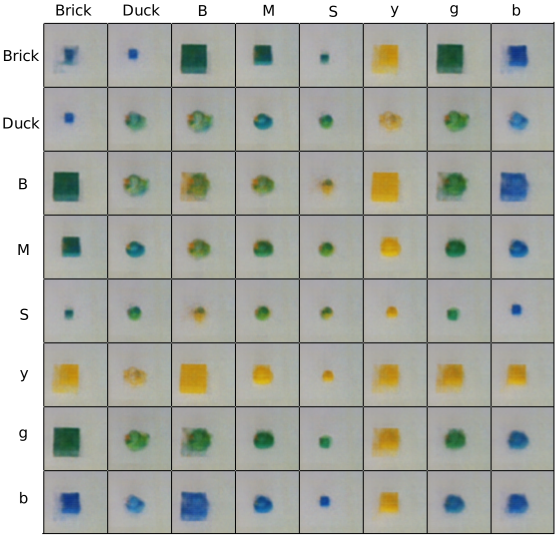
\includegraphics[width=0.7\textwidth]{Figs/chapter6/2wordsExemplarBrickDuck.png}
    \caption{Images generated using word pairs using the MAE trained using image exemplars.}
    \label{fig:2wordsExemplarBrickDuck}
\end{figure*}

\subsubsection{Image Generation}
\subsubsection{Multilabel Classification}
\subsubsection{Vector Arithematic}

\subsection{Discussion}

%\section{The importance of transfer learning}
%\section{MultiSense 1 dataset}
%\subsection{dataset description}
%\subsection{problem description: image generation from raw speech audio}
%\subsection{network description}
%\subsection{results}
%\subsection{discussion}
\theendnotes